\section{Steganalysis}$First draft$
Steganalysis is the study of detecting information hidden with steganography and if possible, recover that information.
Because of the nature of steganography, it is not always obvious if a file has hidden information or not.
Therefore steganalysis is often used on a large set of files, which are suspected of containing hidden data.
$TODO: add more to intro$

\subsection*{Detection}
Most steganography algorithms are able to hide data without any notable visual impact on images.
It is therefore hard if not impossible to detect if something is hidden by simply looking at the image.
Detection of hidden data is therefore done with statistical tools like looking at histograms, modified and signatures of different steganography algorithms.

\subsubsection*{Histogram}


this is without LSB in figure \ref{fig:HistoWithoutLSB}, and this is with LSB in figure \ref{fig:HistoWithLSB}

\begin{figure}
	\centering
	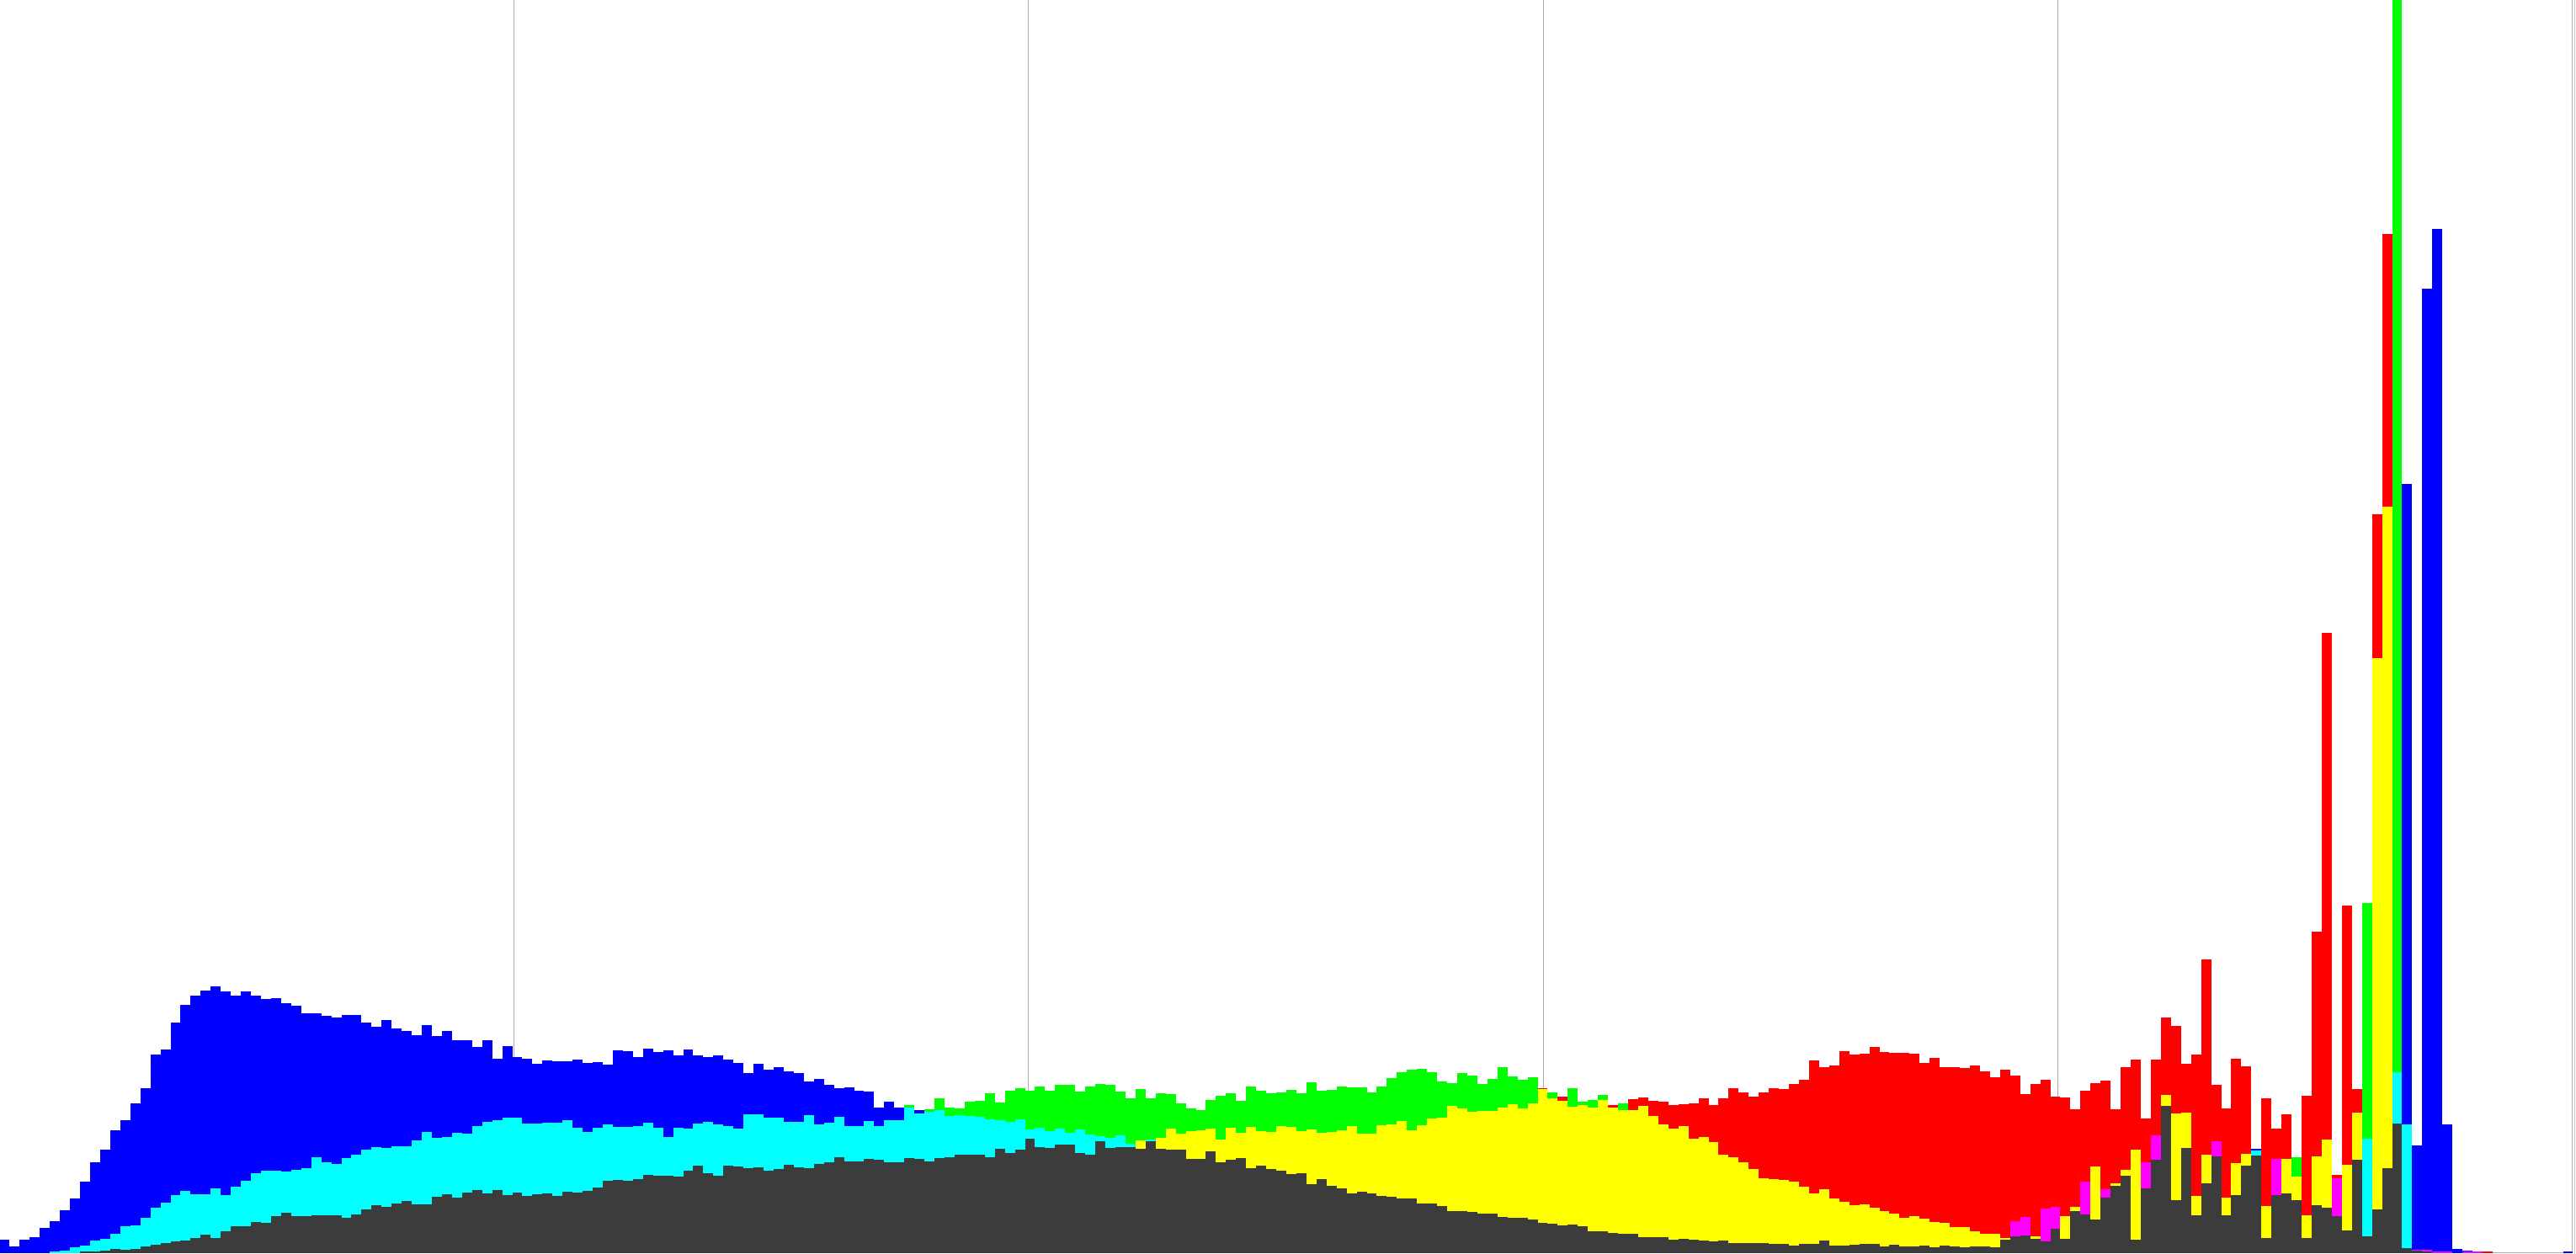
\includegraphics[width=1\textwidth]{figures/HistoLSBCat.png}
	\caption{Colour Histogram of image without hidden data.}
	\label{fig:HistoWithoutLSB}
\end{figure}

\begin{figure}
	\centering
	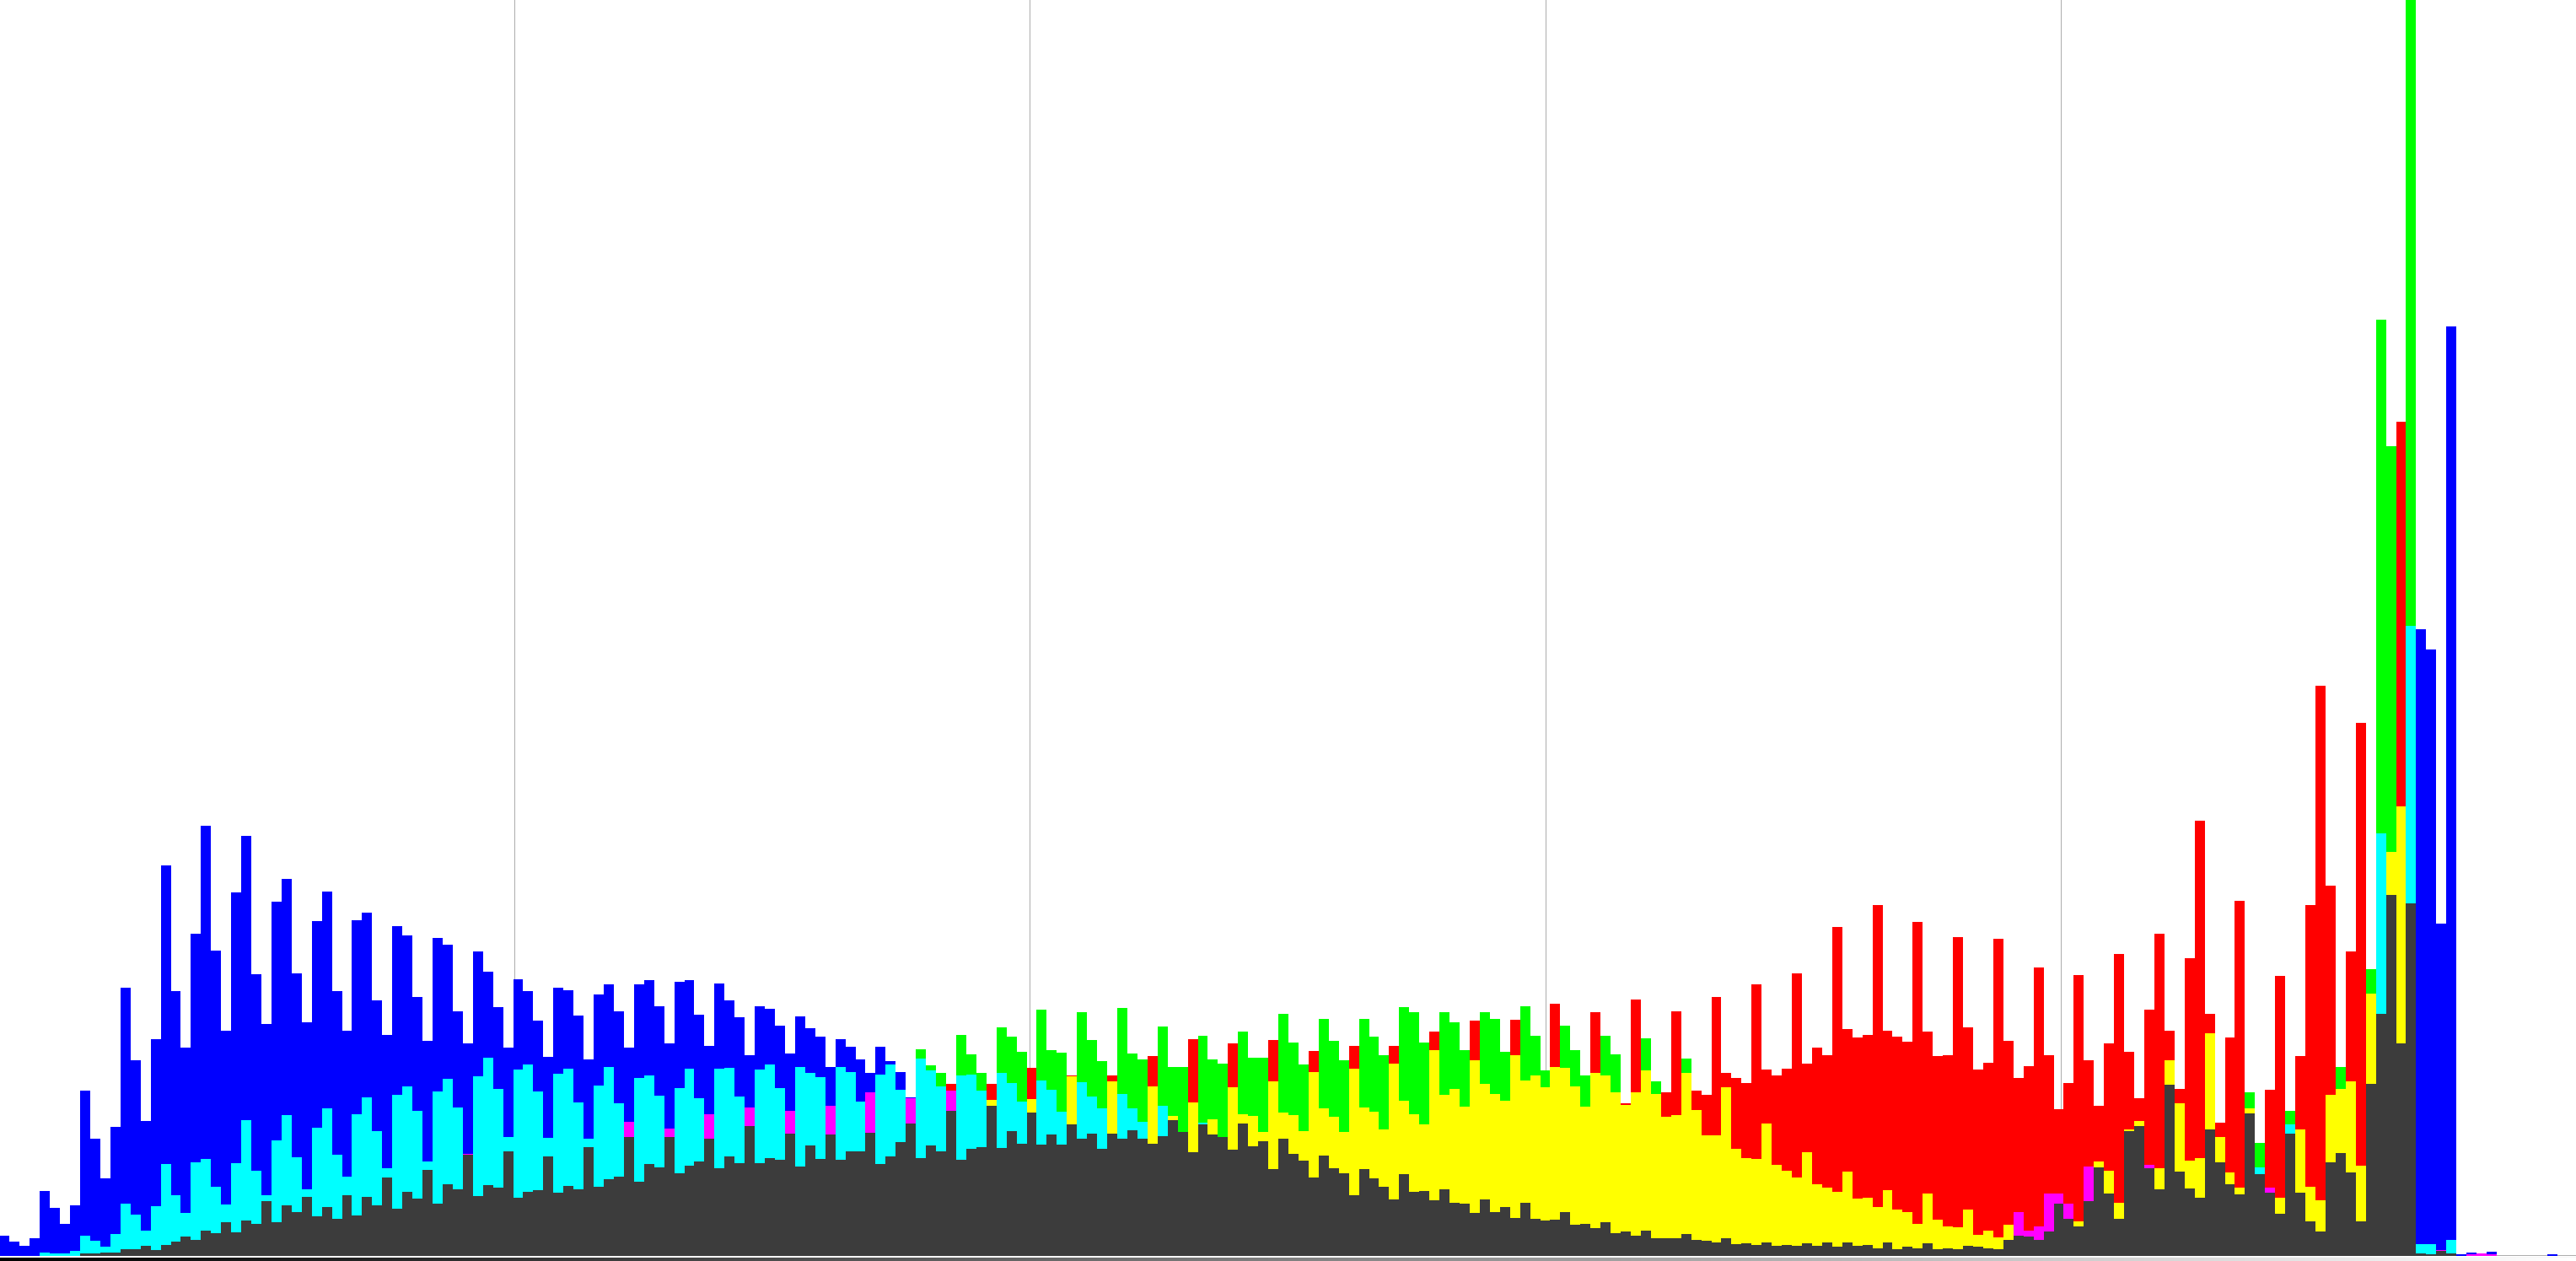
\includegraphics[width=1\textwidth]{figures/HistoLSBCatEncrypted.png}
	\caption{Colour Histogram of image containing secret image hidden with LSB.}
	\label{fig:HistoWithLSB}
\end{figure}